\documentclass[border=8pt]{standalone}
\usepackage[T1]{fontenc}
\usepackage{lmodern,amsmath,amssymb,tikz}
\usetikzlibrary{arrows.meta,decorations.markings,calc}
\definecolor{branch}{RGB}{185,83,30}
\definecolor{direct}{RGB}{37,82,156}
\definecolor{merged}{RGB}{109,57,133}
\tikzset{v/.style={circle,fill=black,inner sep=1.6pt},edge/.style={line width=.8pt,postaction={decorate},decoration={markings,mark=at position .5 with {\draw[line width=.8pt,fill=white] (-.35,-.14) rectangle (.35,.14);},mark=at position .80 with {\arrow{Stealth[length=1.5mm]}}}},source/.style={-{Stealth[length=1.7mm]},line width=.75pt},box/.style={fill=white,inner sep=1.3pt},reduce/.style={-{Stealth[length=2mm]},line width=.9pt}}
\begin{document}
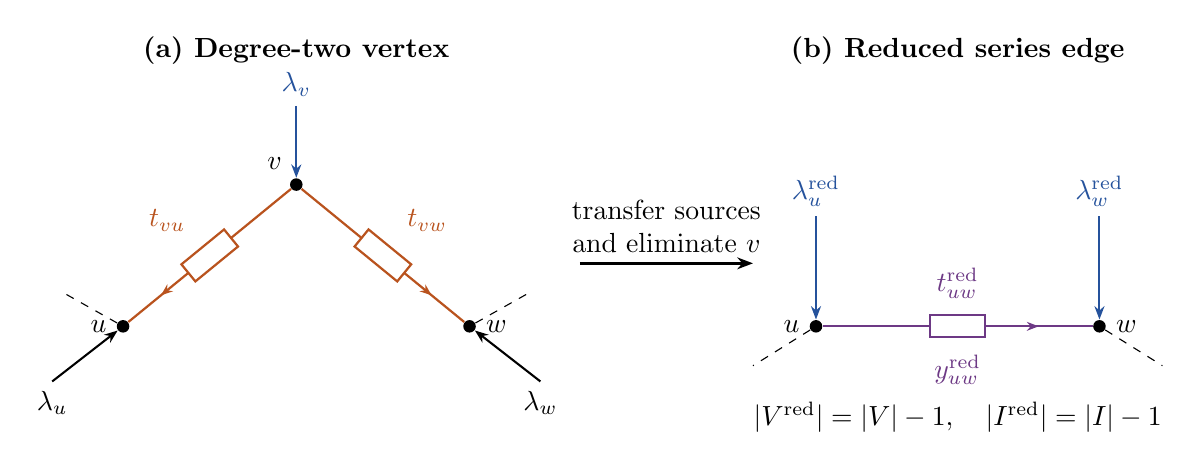
\begin{tikzpicture}[font=\fontsize{10}{12}\selectfont]

\node[font=\bfseries] at (2.2,3.5) {(a) Degree-two vertex};
\node[v,label=left:$u$] (u) at (0,0) {};
\node[v,label=above left:$v$] (v) at (2.2,1.8) {};
\node[v,label=right:$w$] (w) at (4.4,0) {};
\draw[edge,branch] (v)--node[box,above left=2.5mm]{$t_{vu}$} (u);
\draw[edge,branch] (v)--node[box,above right=2.5mm]{$t_{vw}$} (w);
\draw[source,direct] (2.2,2.8)--(v);\node[above,direct] at (2.2,2.8) {$\lambda_v$};
\draw[source] (-.9,-.7)--(u);\node[below] at (-.9,-.7) {$\lambda_u$};
\draw[source] (5.3,-.7)--(w);\node[below] at (5.3,-.7) {$\lambda_w$};
\draw[dashed] (u)--(-.8,.45);\draw[dashed] (w)--(5.2,.45);
\draw[reduce] (5.8,.8)--node[above,align=center]{transfer sources\\and eliminate $v$}(8,.8);
\node[font=\bfseries] at (10.6,3.5) {(b) Reduced series edge};
\node[v,label=left:$u$] (ru) at (8.8,0) {};
\node[v,label=right:$w$] (rw) at (12.4,0) {};
\draw[edge,merged] (ru)--node[box,above=3mm]{$t_{uw}^{\mathrm{red}}$}node[box,below=3mm]{$y_{uw}^{\mathrm{red}}$}(rw);
\draw[source,direct] (8.8,1.4)--(ru);\node[above,direct] at (8.8,1.4) {$\lambda_u^{\mathrm{red}}$};
\draw[source,direct] (12.4,1.4)--(rw);\node[above,direct] at (12.4,1.4) {$\lambda_w^{\mathrm{red}}$};
\draw[dashed] (ru)--(8,-.5);\draw[dashed] (rw)--(13.2,-.5);
\node at (10.6,-1.15) {$|V^{\mathrm{red}}|=|V|-1,\quad |I^{\mathrm{red}}|=|I|-1$};

\end{tikzpicture}
\end{document}
